\section{Aufbau und Durchf"uhrung}
	\label{sec:durchf"uhrung}
	F"ur den Versuch stand ein He-Ne-Laser, ein gr"o"senverstellbarer Einfachspalt , ein gr"o"senverstellbarer Doppelspalt, ein lichtempfindlicher Detektor auf einer mechanischen Schiene sowie ein Amperemeter zur verf"ugung.

	\subsection{Messaufgaben}
		\begin{enumerate}
			\item \label{aufg_1} Punktweises Ausmessen der Beugungsfigur des Einfachspalts (50 Messpunkte). Anschlie"sendes bestimmen der Spaltbreite $b$ und ausmessens der Spaltbreite $b$ mit dem Mikroskop.

			\item \label{aufg_2} Wie \ref{aufg_1} aber mit variablem Einfachspalt und ohne Mikroskop. 

			\item \label{aufg_3} Wie \ref{aufg_1} aber mit festem Doppelspalt und anschlie"sendem Vergleich mit der theoretischen Verteilung des Einfachspaltes.
		\end{enumerate}

	\subsection{Durchf"uhrung}
		\label{sec:durchfuehrung}
		\subsubsection{Messungen}
			\label{sec:messung}

			Der Laser beleuchtet mit einer Wellenl"ange von $\lambda = \SI{633}{\nano \meter}$ wie in \ref{Versuchsaufbau} beschrieben einen ca. $20 - 200 \SI{}{\micro \meter}$ breiten Parallelspalt. Ein lichtempfindlicher Detektor befindet sich in etwa $100 - 120 \SI{}{\centi \meter}$ entfernung vom Spalt, welcher senkrecht zur optischen Achse verstellbar ist.

			\begin{figure}[h]
					\centering
					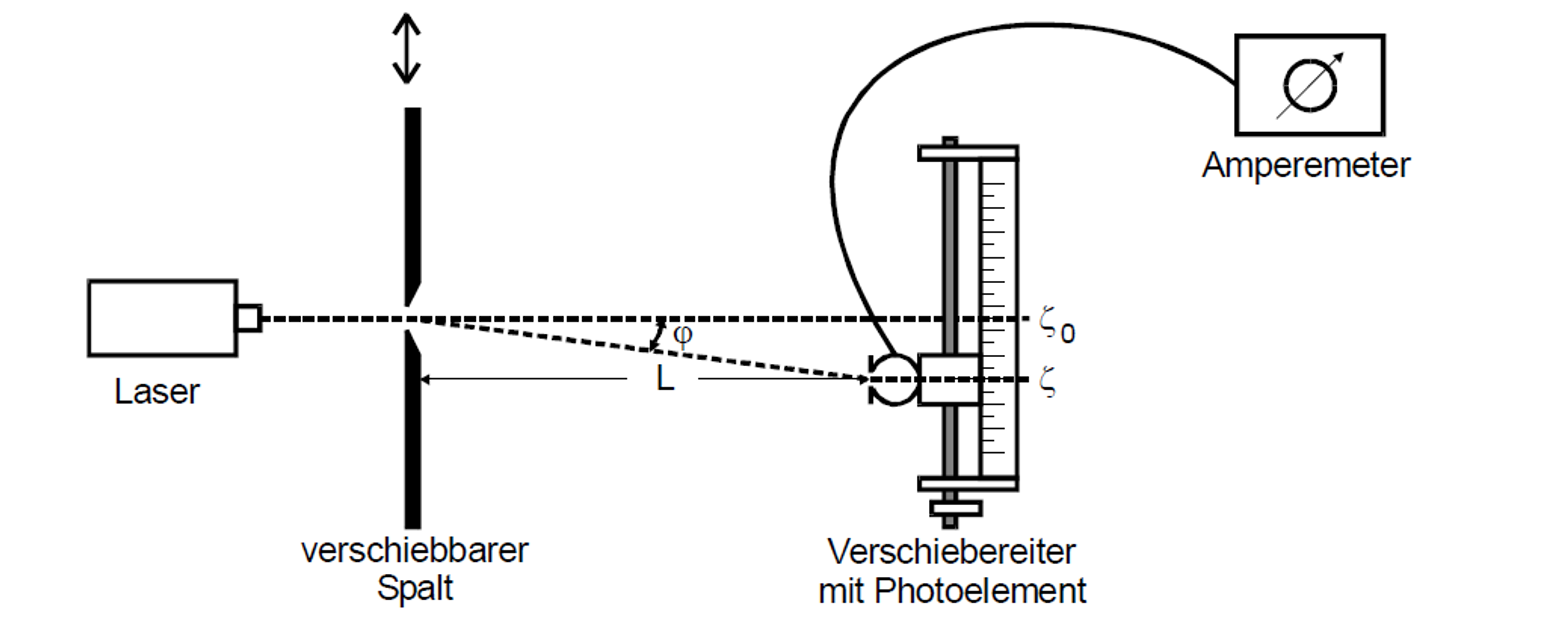
\includegraphics[width = 14cm]{Versuchsaufbau.png}
					\caption{Abb.?}
					\label{Versuchsaufbau}
			\end{figure}

			Anfangs muss die Apparatur justiert werden. Daf"ur wird der Laser fixiert und die h"ohe des Detektors in Mittelstellung so ausgerichtet, dass der Laserstrahl genau auf den Sensor trifft. Anschlie"send wird der f"ur die Messung ben"otigte Spalt in die daf"ur vorgesehene Vorrichtung gesteckt und so daran gedreht bis das Hauptmaximum mittig vom Sensor erfasst wird und die n-ten Nebenmaxima links und rechts des Hauptmaximas in etwa die gleiche Intensit"at haben.

			Nun kann die Intensit"at der Beugungsfigur abh"angig von der Detektorstellung gemessen werden. Dabei wird "uber einen Verschiebeweg von $\SI{50}{\milli\meter}$ die Intensit"at punktweise gemessen. Die genaue Position kann an der Skala der Schiene abgelesen werden. Ein Strich entspricht einem $\SI{}{\centi \meter}$, genauso wie eine Trommelumdrehung. Auf der Trommel kommt eine Skala hinzu, welche in $\SI{}{\micro \meter}$ ablesbar ist.


			Aus der Position des Detektors l"asst sich der Beugungswinkel $\varphi$ aus der Detektorstellung $\zeta$ bestimmen. Dies ist notwendig um die aufgenommene Intensit"atskurve $I(\zeta)$ mit der dem nach ?????? berechneten Verlauf $I(\varphi)$ vergleichen zu k"onnen.

			Es gilt:

			\begin{equation}
				\varphi \approx \tan{\varphi} = \frac{\zeta - \zeta_0}{L}
			\end{equation}

			Dabei ist $\zeta_0$ die Detektorstellung f"ur den ungebeugten Strahl und $L$ der Abstand des Spalts zur Detektoblende.

			F"ur den Doppelspalt wird genauso vorgegangen.

			\newline

			Zu beachten ist, dass auch bei abgeschaltetem Laser bereits ein sogenannter Dunkelstrom $I_{\text{du}}$ flie"st, welcher daher bei abgedeckter Detektorblende gemessen werden muss.

		\subsubsection{Messung des Abstands per Mikroskop}
			\label{sec:messung_mikro}

			Zun"achst muss das Mikroskop geeicht werden, damit die Breite $b$ des Spalts ausgemessen werden kann. Dies geschieht mithilfe eines Objektmikrometers. Dies ist eine Glasplatte mit einge"atzter Mikrometerskala. In der Brennebene des Okulars liegt eine Skala mit willk"urlicher Teilung. 

			Nach der Fokussierung auf die Skala das Objektmikrometer k"onnen die Skalen verglichen werden und so die Teilung in $\SI{}{\micro \meter}$ ausgedr"uckt werden.
